\documentclass[11pt]{article}
% Use this command to override the default ACM copyright statement
% (e.g. for preprints).  Consult the conference website for the
% camera-ready copyright statement.

% Load basic packages
\usepackage{balance}  % to better equalize the last page
\usepackage{graphicx} % for EPS, load graphicx instead
\graphicspath{{images/}}
\usepackage{txfonts}
\usepackage{times}    % comment if you want LaTeX's default font
\usepackage[pdftex]{hyperref}
\usepackage{color}
\usepackage{textcomp}
\usepackage{booktabs}
\usepackage{ccicons}
\usepackage{todonotes}
\usepackage{csquotes}
\usepackage{url}
\usepackage{pdfpages}
\usepackage{times}
\usepackage[margin=1in]{geometry}
\usepackage{float}

% llt: Define a global style for URLs, rather that the default one
\makeatletter
\def\url@leostyle{%
  \@ifundefined{selectfont}{\def\UrlFont{\sf}}{\def\UrlFont{\small\bf\ttfamily}}}
\makeatother
\urlstyle{leo}

% To make various LaTeX processors do the right thing with page size.
\def\pprw{8.5in}
\def\pprh{11in}
\special{papersize=\pprw,\pprh}
\setlength{\paperwidth}{\pprw}
\setlength{\paperheight}{\pprh}
\setlength{\pdfpagewidth}{\pprw}
\setlength{\pdfpageheight}{\pprh}

% Make sure hyperref comes last of your loaded packages, to give it a
% fighting chance of not being over-written, since its job is to
% redefine many LaTeX commands.
\definecolor{linkColor}{RGB}{6,125,233}
\hypersetup{
  pdftitle={Programming languages of cities},
  pdfauthor={LaTeX},
  pdfkeywords={},
  bookmarksnumbered,
  pdfstartview={FitH},
  colorlinks,
  citecolor=black,
  filecolor=black,
  linkcolor=black,
  urlcolor=linkColor,
  breaklinks=true,
}

\pagenumbering{arabic}  % Arabic page numbers for submission.  Remove this line to eliminate 

\setcounter{secnumdepth}{3} % Automatically adds section numbers

% Beginning of document.
\begin{document}

\title{Assigning programming languages to geographic locations based on the activities of GitHub users}

\author{
   Gelera, Rodney \\University of Victoria
   \and
   McCulloch, Kaileen \\University of Victoria
   \and
   Warwick, Nick \\University of Victoria
}

\maketitle

\tableofcontents
\listoffigures
\newpage

\begin{abstract}
Data has never before been generated at such high speeds. With the ever increasing volume of data becoming available every second, it has become more and more challenging to find meaningful information. Data mining and data visualization are two tools that can help solve this problem. In this paper we discuss the effectiveness of visualization as a data mining tool. We use a classification technique to simplify information and a visualizer as a quick and easy evaluation method. In order to explore these techniques we  use GitHub user data to explore the use of programming languages according to geographic locations. We have scraped GitHub user profiles to get a location and a programming language for each user. From that we can classify each unique geographic location with a single programming language then our visualization tool allows us to explore the geographic distribution of language usage. There is a vast variety of development platforms available, selecting which tools to use can be a challenge. Whether you are a professional looking to stay in the game in this competitive climate or a person just starting their career in tech, looking at the language of choice in your area will help you make a more informed decision.

\end{abstract}

\section{Introduction}
Fundamentally, data mining is an information extraction technique for identifying patterns and trends in large datasets. It is used to derive conclusions from datasets where manual searching is not feasible, due to memory or time constraints, or the raw data is visually incomprehensive. There is a broad range of techniques and with the surge of /texttt{big data}, it is becoming even more important.

\section{Related Work?}

\section{Data Collection}

When researching a way to gather data off GitHub user profiles, we found that GitHub has their own API for this\footnote{https://developer.github.com/v3/}. However, it had a rate limit of 60 requests. There are three requests we would need to use if we were to use the GitHub API:

\definecolor{r}{rgb}{1,0,0}
\definecolor{b}{rgb}{0,0,1}
%{\fontfamily{cmr}\selectfont
\begin{itemize}
   \item{\texttt{GET /users?since=0}}
   \begin{itemize}
	\item{Returns a list of 30 users with limited information starting from specified id}
	\item{ [\\
	\texttt{
		\{\\
		\textcolor{r}{"login"}: \textcolor{b}{"octocat"},\\
		\textcolor{r}{"id"}: \textcolor{b}{1},\\
		\textcolor{r}{"avatar\_url"}: \textcolor{b}{"https://github.com/images/error/octocat\_happy.gif"},\\
		\textcolor{r}{"gravatar\_id"}: \textcolor{b}{""},\\
		\textcolor{r}{"url"}: \textcolor{b}{"https://api.github.com/users/octocat"},\\
		\textcolor{r}{"html\_url"}: \textcolor{b}{"https://github.com/octocat"},\\
		\textcolor{r}{"followers\_url"}: \\\textcolor{b}{"https://api.github.com/users/octocat/followers"},\\
		\textcolor{r}{"following\_url"}: \\\textcolor{b}{"https://api.github.com/users/octocat/following\{/other\_user\}"},\\
		\textcolor{r}{"gists\_url"}: \\\textcolor{b}{"https://api.github.com/users/octocat/gists\{/gist\_id\}"},\\
		\textcolor{r}{"starred\_url"}: \\\textcolor{b}{"https://api.github.com/users/octocat/starred\{/owner\}\{/repo\}"},\\
		\textcolor{r}{"subscriptions\_url"}: \\\textcolor{b}{"https://api.github.com/users/octocat/subscriptions"},\\
		\textcolor{r}{"organizations\_url"}: \\\textcolor{b}{"https://api.github.com/users/octocat/orgs"},\\
		\textcolor{r}{"repos\_url"}: \\\textcolor{b}{"https://api.github.com/users/octocat/repos"},\\
		\textcolor{r}{"events\_url"}: \\\textcolor{b}{"https://api.github.com/users/octocat/events\{/privacy\}"},\\
		\textcolor{r}{"received\_events\_url"}: \\\textcolor{b}{"https://api.github.com/users/octocat/received\_events"},\\
		\textcolor{r}{"type"}: \textcolor{b}{"User"},\\
		\textcolor{r}{"site\_admin"}: \textcolor{b}{false}\\
		\},\\
  		\{\\
		...\\
  		\},\\
  		...\\
		\}
		]
   	 }
	}
   \end{itemize}

   \item{\texttt{GET /user}}
	\begin{itemize}
	   \item{Returns information about the given user}
	\end{itemize}
   \item{\texttt{Get /users/:username/repos}}
	\begin{itemize}
	   \item{Returns a list of repositories of the given user}
	   \item{ \{\\
		\texttt{
			  \textcolor{r}{"login"}: \textcolor{b}{"octocat"},\\
			  \textcolor{r}{"id": 1},\\
			  \textcolor{r}{"avatar\_url"}: \textcolor{b}{"https://github.com/images/error/octocat\_happy.gif"},\\
			  \textcolor{r}{"gravatar\_id"}: \textcolor{b}{""},\\
			  \textcolor{r}{"url"}: \textcolor{b}{"https://api.github.com/users/octocat"},\\
			  \textcolor{r}{"html\_url"}: \textcolor{b}{"https://github.com/octocat"},\\
			  \textcolor{r}{"followers\_url"}: \\\textcolor{b}{"https://api.github.com/users/octocat/followers"},\\
			  \textcolor{r}{"following\_url"}: \\\textcolor{b}{"https://api.github.com/users/octocat/following{/other\_user}"},\\
			  \textcolor{r}{"gists\_url"}: \\\textcolor{b}{"https://api.github.com/users/octocat/gists{/gist\_id}"},\\
			  \textcolor{r}{"starred\_url"}: \\\textcolor{b}{"https://api.github.com/users/octocat/starred{/owner}{/repo}"},\\
			  \textcolor{r}{"subscriptions\_url"}: \\\textcolor{b}{"https://api.github.com/users/octocat/subscriptions"},\\
			  \textcolor{r}{"organizations\_url"}: \\\textcolor{b}{"https://api.github.com/users/octocat/orgs"},\\
			  \textcolor{r}{"repos\_url"}: \\\textcolor{b}{"https://api.github.com/users/octocat/repos"},\\
			  \textcolor{r}{"events\_url"}: \\\textcolor{b}{"https://api.github.com/users/octocat/events{/privacy}"},\\
			  \textcolor{r}{"received\_events\_url"}: \\\textcolor{b}{"https://api.github.com/users/octocat/received\_events"},\\
			  \textcolor{r}{"type"}: \textcolor{b}{"User"},\\
			  \textcolor{r}{"site\_admin"}: \textcolor{b}{false},\\
			  \textcolor{r}{"name"}: \textcolor{b}{"monalisa octocat"},\\
			  \textcolor{r}{"company"}: \textcolor{b}{"GitHub"},\\
			  \textcolor{r}{"blog"}: \textcolor{b}{"https://github.com/blog"},\\
			  \textcolor{r}{"location"}: \textcolor{b}{"San Francisco"},\\
			  \textcolor{r}{"email"}: \textcolor{b}{"octocat@github.com"},\\
			  \textcolor{r}{"hireable"}: \textcolor{b}{false},\\
			  \textcolor{r}{"bio"}: \textcolor{b}{"There once was..."},\\
			  \textcolor{r}{"public\_repos"}: \textcolor{b}{2},\\
			  \textcolor{r}{"public\_gists"}: \textcolor{b}{1},\\
			  \textcolor{r}{"followers"}: \textcolor{b}{20},\\
			  \textcolor{r}{"following"}: \textcolor{b}{0},\\
			  \textcolor{r}{"created\_at"}: \textcolor{b}{"2008-01-14T04:33:35Z"},\\
			  \textcolor{r}{"updated\_at"}: "\textcolor{b}{2008-01-14T04:33:35Z"}\\
			}
		\}\\
   	   }
	\end{itemize}
\end{itemize}

We predicted that the rate limit was going to be a problem so we looked for alternative solutions such as scraping data directly off the HTML. We found a project on GitHub that did just that. The input for this application takes a GitHub URL such as:
\begin{itemize}
\item{a user profile (ex. https://github.com/username)}
\item{a user's repository page (ex. https://github.com/username?tab=repositories)}
\end{itemize}

With this scraper, we wouldn’t have to worry about the rate limitation when requesting for information on GitHub users. One problem we had with it is that it was not updated to the latest GitHub UI. Being an open source project, we were able to manually fix the parts of the scraper that returns information that we needed.

For both solutions, we would still need a list of users to pass into. The only way we would be able to get this list of users is the \texttt{GET /users} request from the GitHub API. With the rate limit, we were able to get 1800 users per hour with 60 requests. The GitHub API returns some user information with this request, but not the information we need such as “location”, thus, the reason we use the scraper to get user information. We did this 13 times to gather a list of 23400 usernames.

The GitHub API returns JSON data with, among other things, a user’s geographic location and programming language. Unfortunately, the API has a request limitation of 60 requests per hour. Each request return informations for 30 users. We retrieved a total of 23400 user profiles. Therefore, this wasn’t a very efficient process.

      \subsection{Determining user location}
GitHub allows users to next their location as a free-form text. This can be problematic for getting exact coordinates for a user's location. Google Maps has a Geocoding API which converts text strings of geographic locations into latitudinal and longitudinal coordinates. Unfortunately this API has a usage limitation of 2,500 free requests per day.

\section{Data Pre-processing}

th a working scraper and a list of usernames, we created a script that uses our modified scraper to get the user’s location and most used programming language based on their repositories. We skipped users that did not set a location, organizations and users that have returned a 404 error. This gave us a final 10241 users, 43.7% of our initial list of users. This may have been due to not many people setting locations on their profile.

GitHub allows users to set their location as a free-form text. This can be problematic for getting exact coordinates for a user's location. Google Maps has a Geocoding API which converts text strings of geographic locations into latitudinal and longitudinal coordinates. Unfortunately this API has a usage limitation of 2,500 free requests per day. With a paid API key, we were able to exceed this limit. The downside to using this API is that we will only be able to get coordinates for whatever the user sets as their location. It can be as specific as a street address, or it can be as vague as just a country name. It may not be a real location at all. The Geocoder API tries its best to find the best matching coordinates. For example, if a user sets its location to “Canada”, the coordinates returned are in the middle of northern Saskatchewan. These results may not be 100% accurate but it gives the general location of where the user is.

After getting the user’s coordinates, the script finds the user’s most used language. GitHub classifies a repository as a certain programming language based on how many lines of code that project contains. Our script looks at this attribute for each of the user’s repository and finds the most frequent programming language used by the user. For ties, all languages tied are kept for the moment. Once we have the user’s coordinates and the user’s most used programming language(s), the script adds the user data to a GeoJSON formatted JSON.

The user data needed to be aggregated on a geographic location basis, in order to class each unique location by a single programming language. This was a multi-step process. Firstly, all users with a same geographic coordinate were merged into a single instance. During the merge a dictionary of programming languages for each location was maintained which tallied the number of users using each language. For users with multiple languages, that user would count once for each one of their used language. The language used by the most users was then chosen as the winning language. If languages were tied for most used, an arbitrary language, other than 'NULL', was selected as the winning language. Obviously this is a very naive way of approaching this problem. A better method would be to apply a weight to each usage. To demonstrate this consider a simple case of a geographic location which has 'Ruby' and 'JavaScript' tied for most used with one user each. Now say the JavaScript user only used JavaScript in one project and the Ruby user used Ruby in hundreds of projects. In this case it would make more sense to classify the location as Ruby since it's used in more projects for that area. Applying a usage weighting would do exactly that, whereas, with the arbitrary selection each language has a 50\% chance of being selected.

Additionally, the data retrieved in the \textit{Data Retrieval} step needed to be converted into a geojson format in order to be input into the \textit{Data Visualizer}. Conversion from json to geojson was a simple matter of adding one additional geometry feature, namely, 'coordinates'.

\section{Data Visualization}
The data visualization portion of our project involved creating a method for reading our data and displaying it in on a map, representing the location of a point correctly such that it matches its respective coordinates. We also had to figure out a method for representing the respective programming language of a given data point. We decided to encode programming languages as colours, since it provided a wide range of possible values to represent the 200 languages we were tracking, in addition, GitHub already represents different programming languages as colours, so it seemed fitting.
After researching various methods for doing data visualization in JavaScript, we decided to use Mapbox GL JS, a JavaScript library that renders interactive maps using WebGL (Web Graphics Library)\footnote{https://www.mapbox.com/mapbox-gl-js/api/}. WebGL js a JavaScript API that allows for the rendering of interactive 2D and 3D graphics in a compatible web browser without the need for plugins\footnote{https://developer.mozilla.org/en-US/docs/Web/API/WebGL\_API}. The use of WebGl allows for extremely fast and smooth interactions.

\begin{figure}[H]
\centering
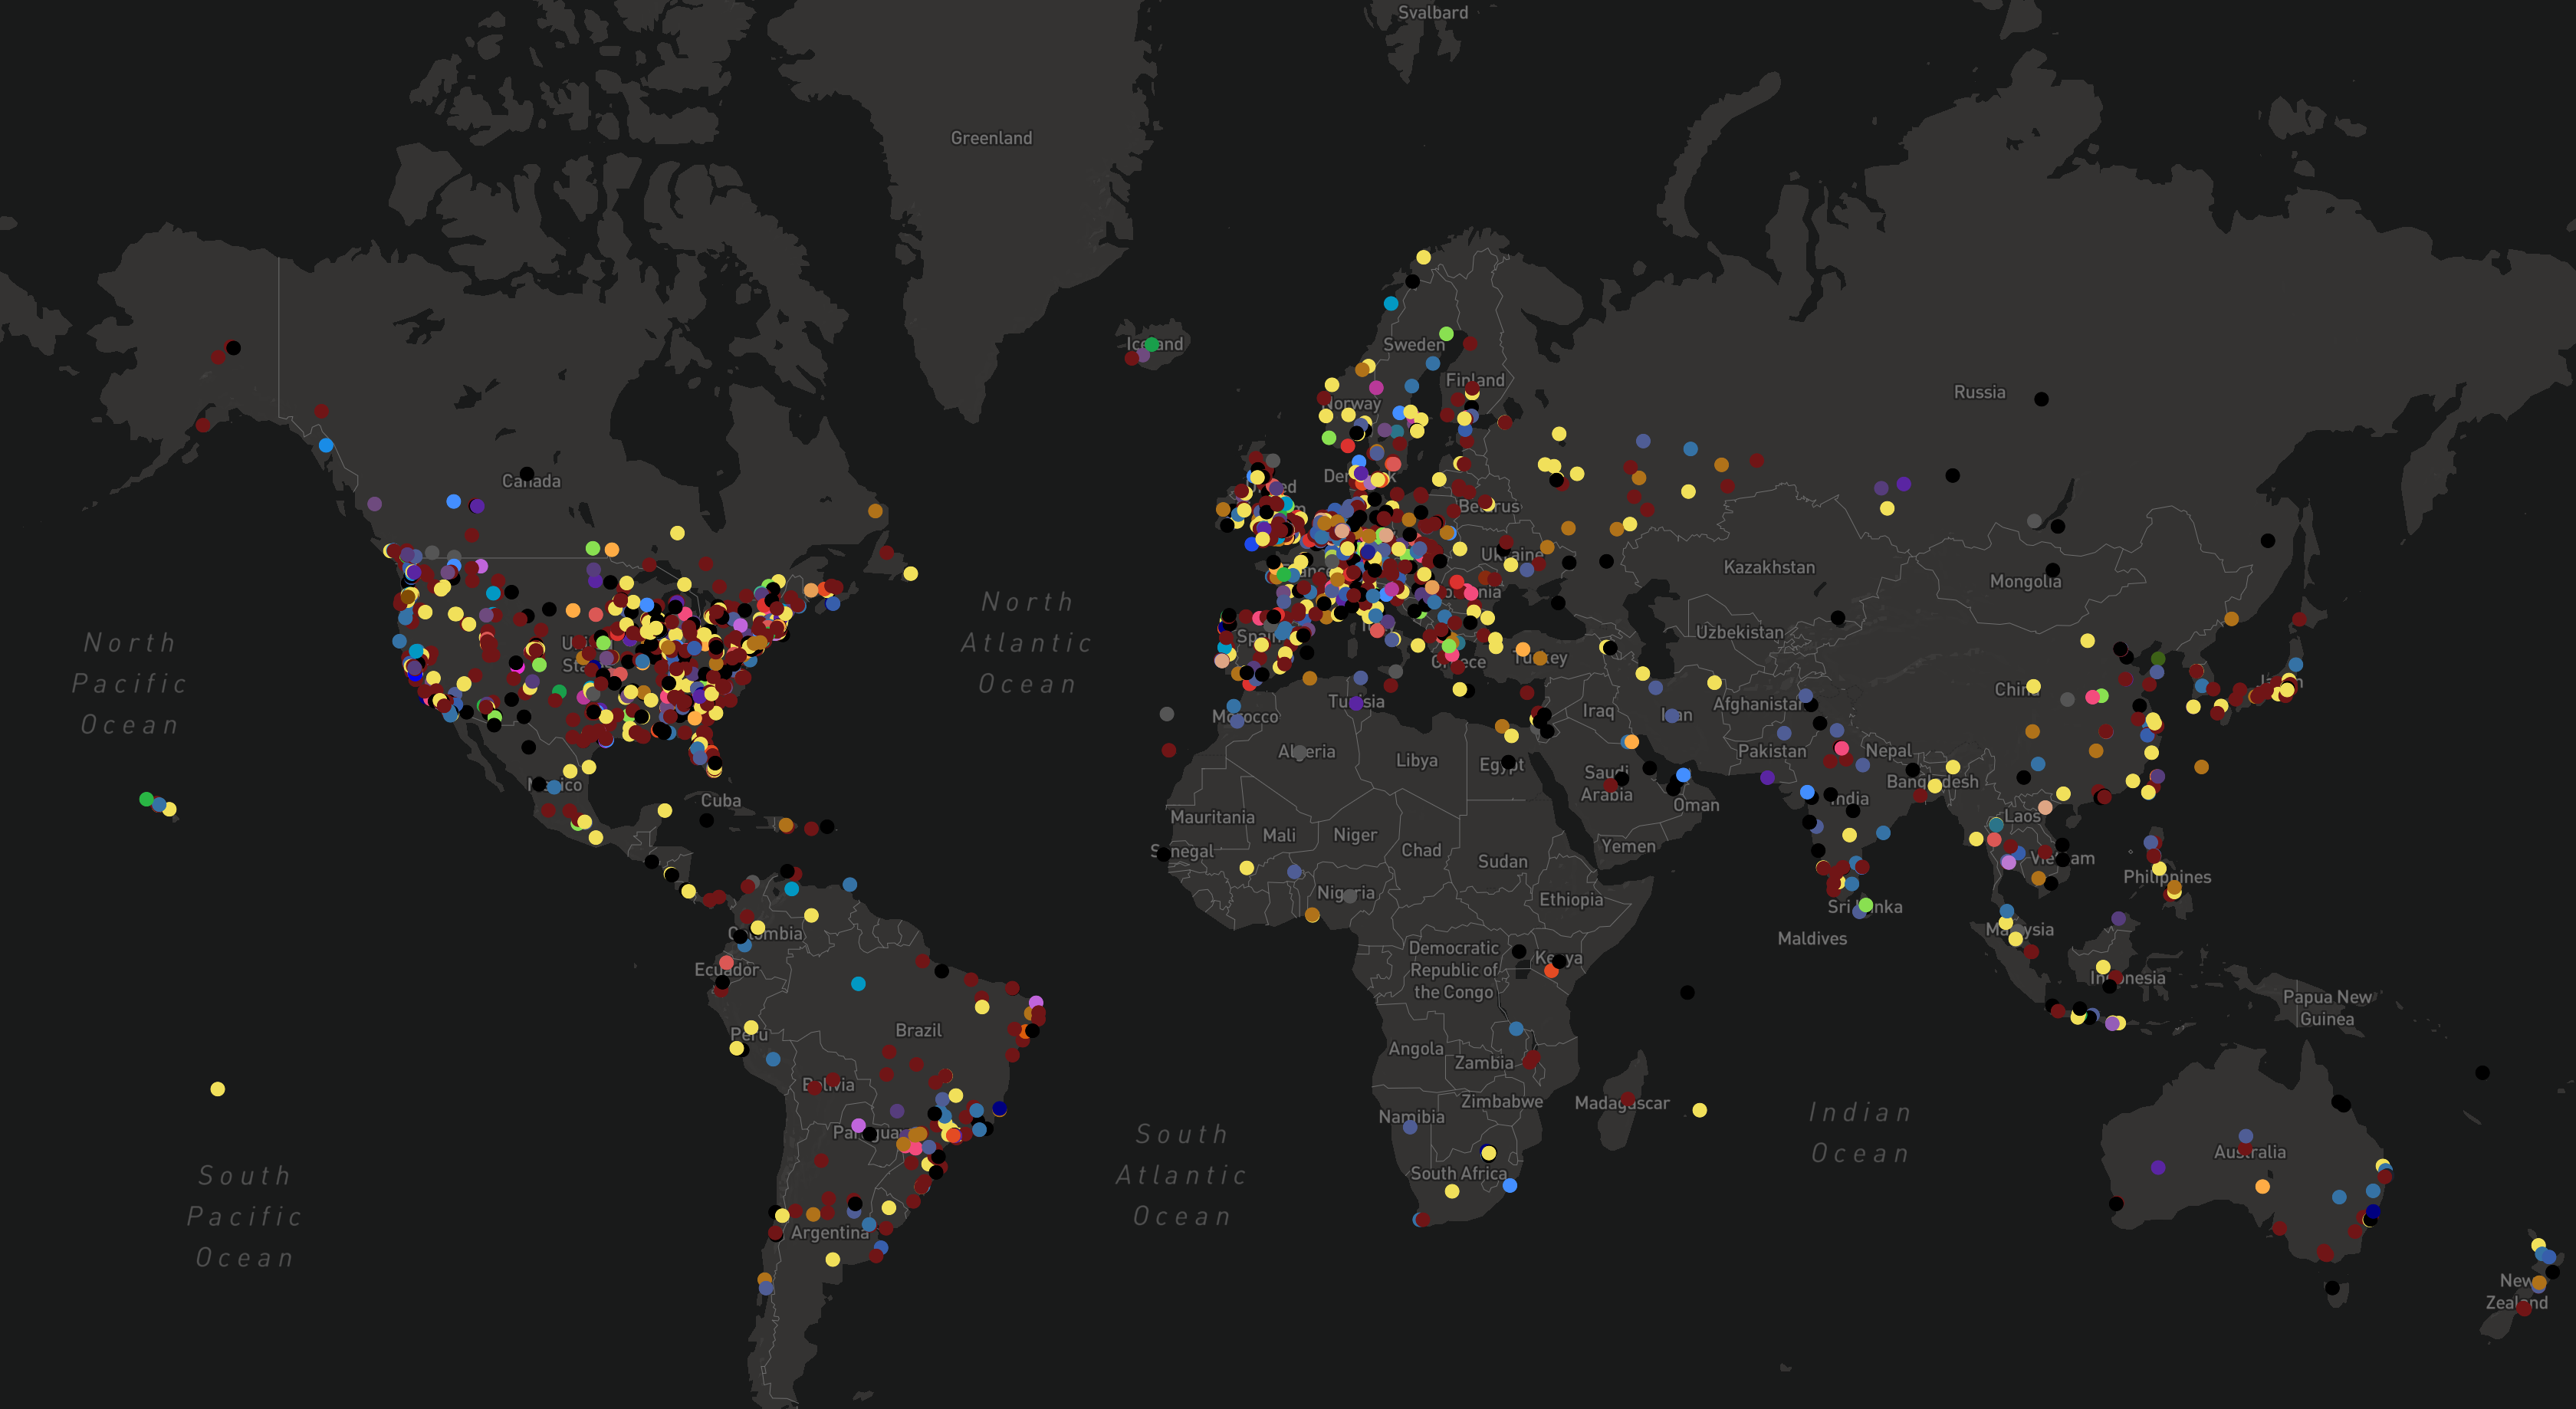
\includegraphics[scale=0.25]{Visualizer.png}
\caption{Map of all languages}
\label{fig:vis}
\end{figure}

Figure \ref{fig:vis} shows a map with all of our data points shown. From first glance, it is clear that the yellow dots (JavaScript) and the dark red dots (Ruby), are the most prevalent. We see clusters of data points which represent geographic locations with large numbers of github users, these clusters for the most part are in locations where we would expect them, i.e. on the east and west coast of the US, as well as in Europe. 

When representing all of the data points on a single map, it is hard to see any correlation between geographic location and popular programming languages. However, when filtering and plotting data points for specific languages, it becomes easier to see potential trends in the data.

\begin{figure}[H]
\centering
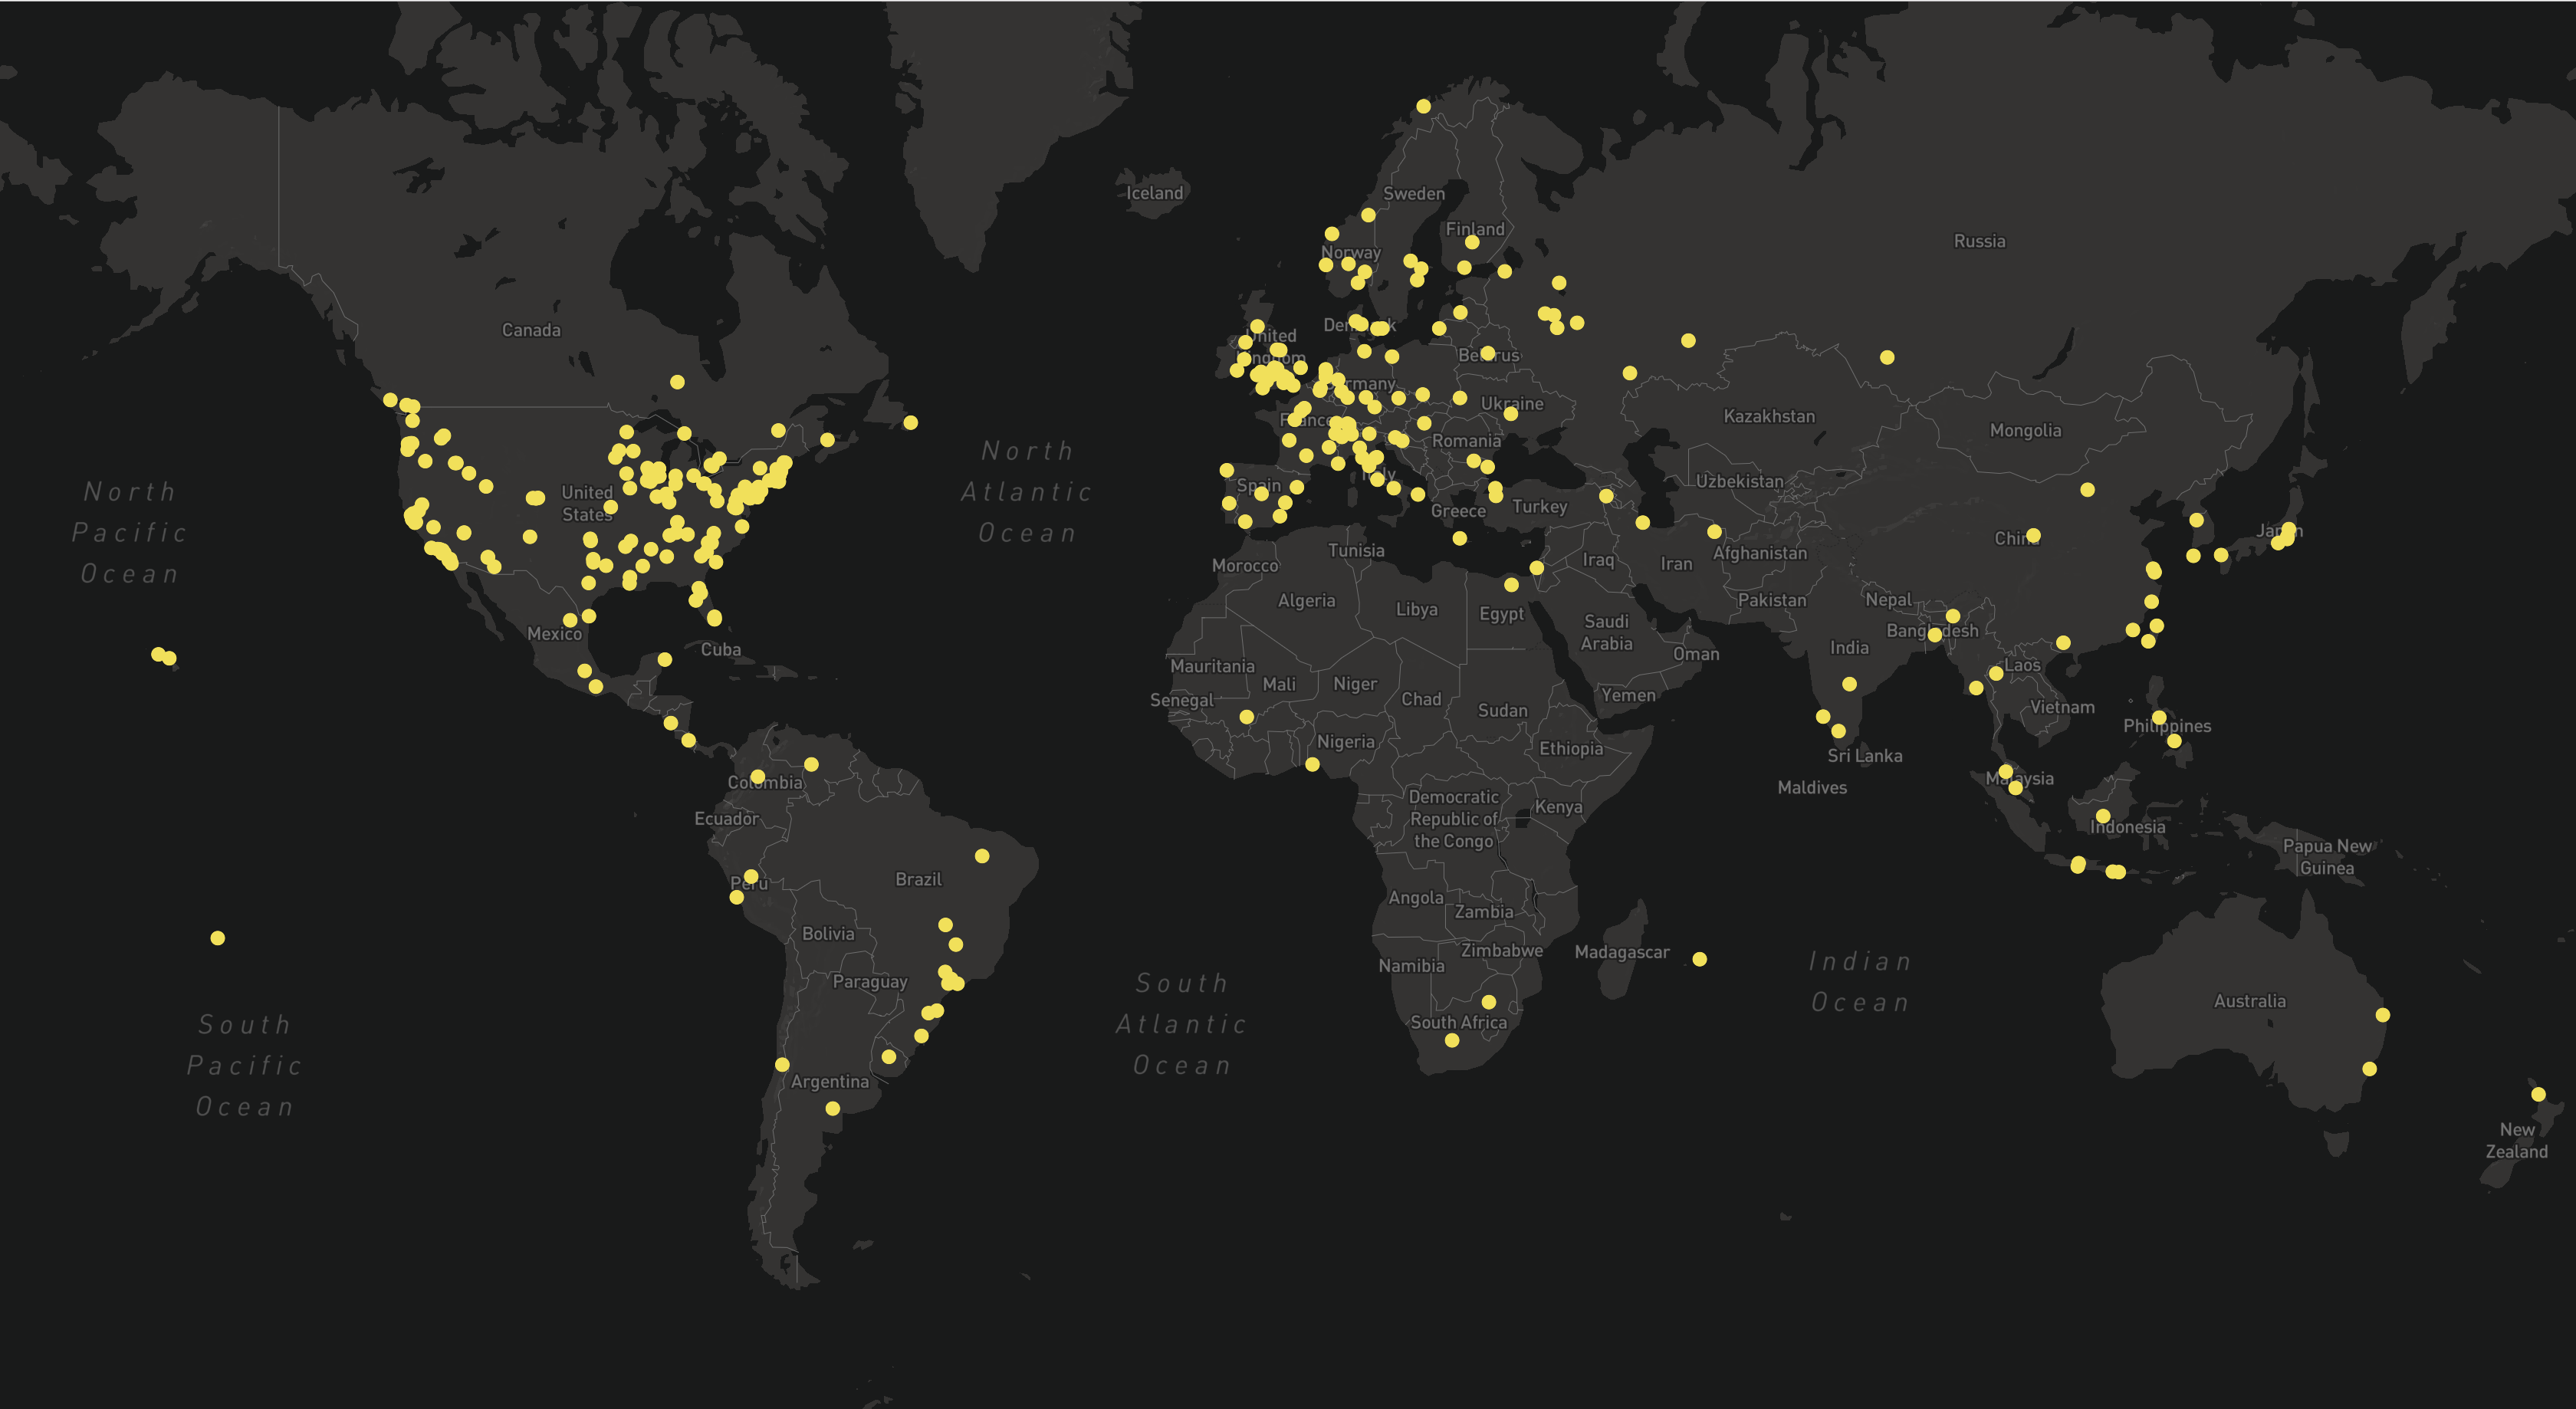
\includegraphics[scale=0.25]{JavaScript.png}
\caption{Map of JavaScript}
\label{fig:js}
\end{figure}

\begin{figure}[H]
\centering
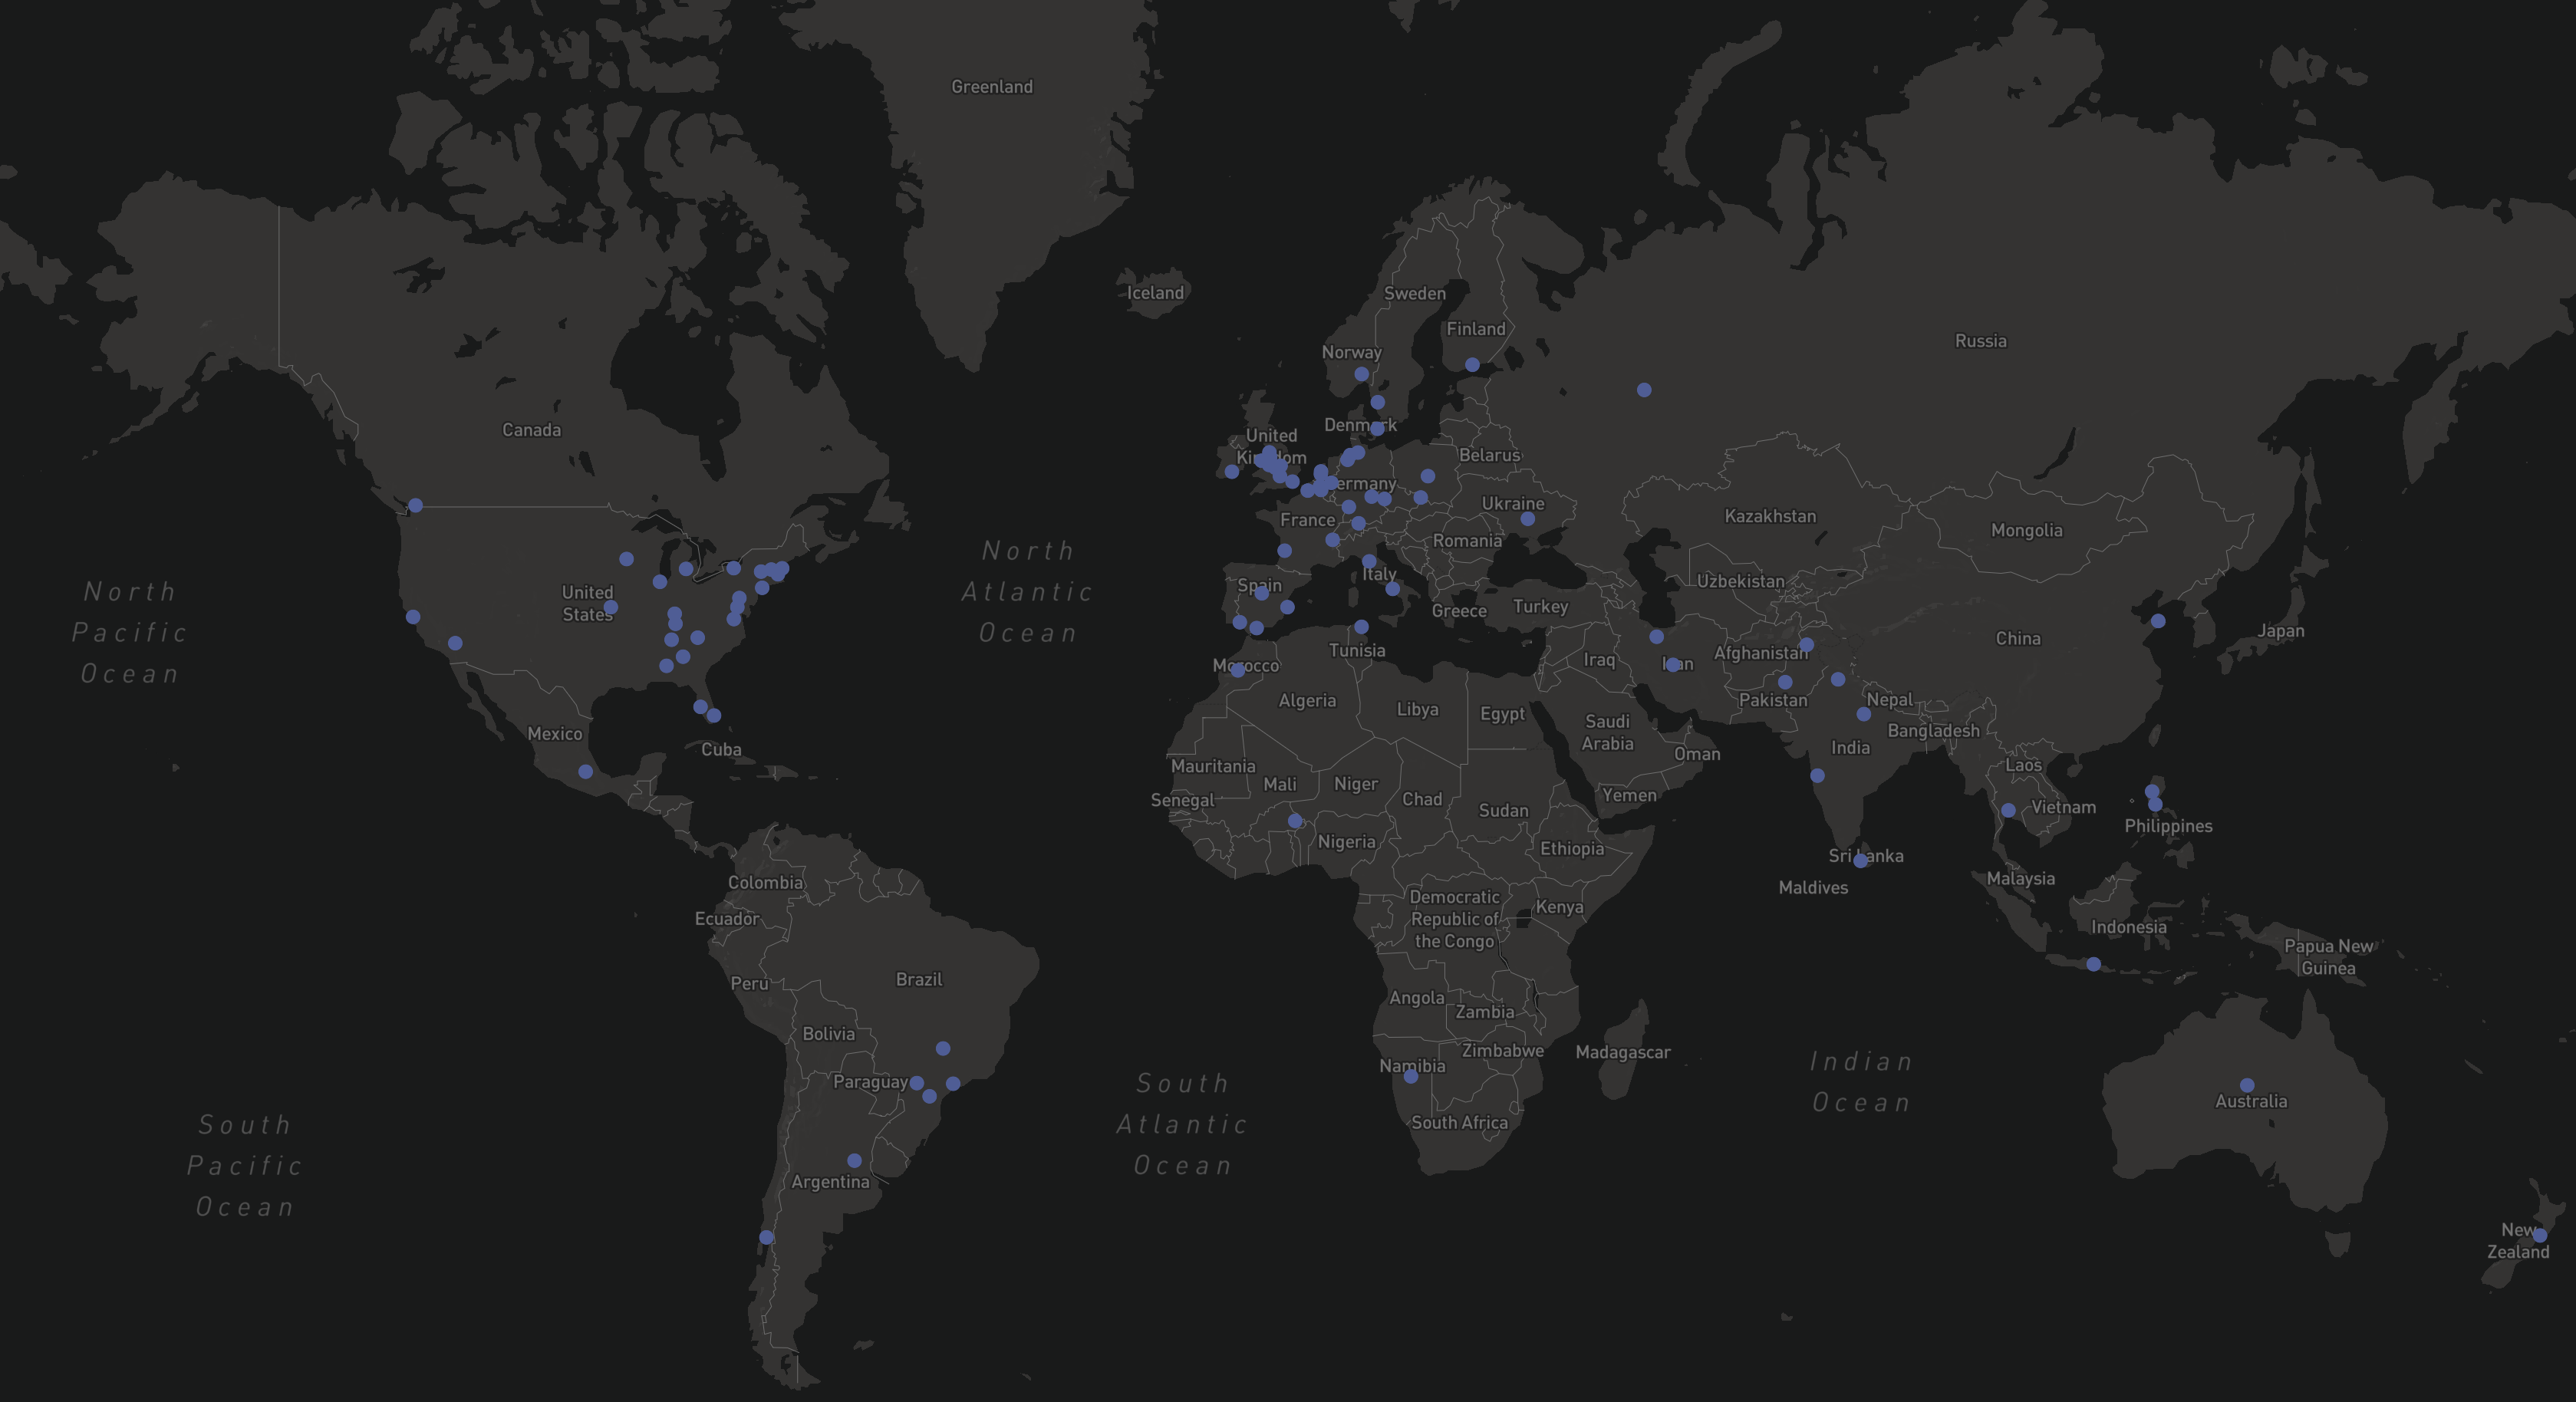
\includegraphics[scale=0.25]{PHP.png}
\caption{Map of PHP}
\label{fig:php}
\end{figure}

Figure \ref{fig:js}, with the yellow dots, represents the use of JavaScript, whereas Figure \ref{fig:php} represents the use of PHP. As you can see, for the most part the languages have similar clusters, however, JavaScript is much more popular on the west coast of the US, whereas PHP has almost no influence in the west. This could be due to the tech hubs in the west coast favouring JavaScript over PHP.

\section{Conclusion}
In conclusion, we found that there does seem to be small trends in programming language popularity (for some languages) potentially related to geographic locations, however, we would need to analyse a larger dataset to confirm our findings. From our visualization we also found that Ruby and JavaScript are the most popular programming languages in North America and Europe, at least according to our dataset. Ultimately, this application helps to show the power of datavisualization in extracting information from large and complex datasets.

\section{Future Work}
There are multiple streams of future work for this project, such as creating a heatmap view rather than plotting points and adding a feature that allows for a timelapse, showing the different trends in programming language usage over time. Using a larger dataset would also be beneficial in getting a more useful visualization.

% REFERENCES FORMAT
% References must be the same font size as other body text.
\bibliographystyle{SIGCHI-Reference-Format}
\bibliography{../../latex_files/refs}
\citation
\pagebreak
\onecolumn
\begingroup


\endgroup

\end{document}

